\chapter{Secure and Scalable Internet-scale Connectivity}
\label{sec:signpost}

In this chapter we explore applications of the SDN technology in connectivity and
naming scalability.  The work is motivated by the user requirement to create a
network federation between its devices.  We call this functionality a
\emph{Personal Cloud}.  Currently, Personal Clouds use third-party Cloud
services as information caches, to bridge the inter-device communication
requirements. Device federation is currently limited due to the connectivity and
naming limitations of the Internet architecture.  This architecture is a
consequence of the connectivity scalability limitations of the Internet, as
discussed in Section~\ref{sec:intro:motivations}. Nonetheless, as users offload
personal information to third-party services, they become subject to privacy
threats and performance degradation.

We argue that end-devices require an adaptable network control architecture, in
order to overcome  connectivity limitations and control their data and
resources.  The network community provides an abundance of free and open
mechanisms, which can be reused dynamically to provide inter-device
connectivity.  We introduce \signpost~\cite{Rotsos14}, a network control plane for end-devices,
capable of delivering continuous and secure connectivity between user devices.
\signpost uses existing network testing approaches to detect network
environment conditions and configures existing software packages to establish
end-to-end connectivity between devices. 

In order to understand the feasibility and performance of the proposed
architecture, we present a strawman implementation of the core control logic and
its integration with a number of network connection and notification services.
Currently, \signpost supports SSH~\mycite{RFC4245}, OpenVPN~\mycite{openvpn},
TOR~\mycite{dingledine2006}, NAT-punch and Privoxy~\mycite{privoxy} 
mechanisms, while it can also propagate Multicast-DNS notifications across
devices.

For the rest of this chapter, we present a preliminary categorisation of
Personal Cloud platforms and, motivated by some key observations, we define the
key design requirements for our
platform~(Section~\ref{sec:signpost-introduction}). Furthermore, we present the
\signpost abstraction~(Section~\ref{sec:sp-signpost}) and
architecture~(Section~\ref{sec:signpost-architecture}), followed by an elaborate
description of a strawman \signpost implementation and an evaluation of its
functionality~(Section~\ref{sec:signpost-evaluation}).  Finally, we conclude with our
observations~(Section~\ref{sec:signpost-conclusion}).

\section{Personal Clouds}\label{sec:signpost-introduction}

The digital revolution of our era has mirrored a large part of our life in the
digital domain. For example, human labour is commonly stored in PDF and word
processing files, while social interactions are partially captured in digital
photo collections.  Effectively, our physical presence has an increasing digital
counterpart, accessible through computing devices.  Nonetheless, the
increase in the adoption of personal computers introduces challenges in the
management of our digital footprint.  Complimentary to personal computers, users
 own and use tablets, smartphones and other purpose-built computing
units (e.g.~home entertainment systems and gaming consoles), while the IoT
paradigm~\mycite{Atzori2010} will extend further.  From a user perspective, each
device fulfils a specific role in managing digital resources, thus requiring
access only to a subset of the user's digital presence, but these roles are fluid.
For example, a smartphone is primarily a communication device,
but end-users may use it as a media player. In the latter case, the smartphone
and the home entertainment system provide similar functionality to the user and
require access to the same subset of his digital presence. As a result, the
transition from a single PC to a multi-device paradigm requires global and
homogeneous access and control mechanisms of digital information and
resources. We define this abstraction as the user's \emph{Personal Cloud}. 

This section presents existing Personal Cloud mechanisms, discusses their
functional limitations~(Section~\ref{sec:sp-approaches}), and defines the core
\signpost goals~(Section~\ref{sec:sp-challenges}). 

\subsection{Approaches} \label{sec:sp-approaches}

Personal Cloud functionality is readily available in a number of applications,
providing a wide range of abstractions. This section provides a simple taxonomy,
based on their architecture. 

\paragraph*{Decentralised Personal Cloud}

The decentralised Personal Cloud application class contains standalone
connectivity mechanisms, managed by end-users.  Computer networks by design 
provide the middleware to enable information and resource sharing between
computers. As a result, the network community provides an extensive collection
of applications and protocols that support Personal Cloud functionality, such as
remote desktop access (e.g.~Remote Frame Buffer protocol~\mycite{RFC6143}), file
sharing (e.g.~NFS~\mycite{RFC1094}; SAMBA file service~\mycite{samba}), remote login
(e.g.~SSH~\mycite{RFC4253}), remote printing (e.g.~IPP~\mycite{RFC2911}).
Such systems employ a client-server architecture and extend the computer
abstraction to include inter-device connectivity.  A user can set-up and manage
sharing services on his personal devices and enhance his computing experience.
Furthermore, the setup complexity of some services has motivated the
development of automation mechanisms like Multicast-DNS, UPnP and ZeroConf,
which allow a user to seamlessly browse and access available services. 

Decentralised Personal Cloud applications provide extensive control over
personal data and strong privacy guarantees. Decentralised approaches are a
popular mechanism for sharing data  within the local network, like the home
network, Nonetheless, Internet-scale deployment of such mechanism faces
significant scalability problems, primarily due to the following three issues:

\begin{itemize}
  \item {\it Connectivity}\/: Decentralised Personal Cloud effectiveness is
    defined by Internet connectivity limitations.  The current Internet
    architecture does not guarantee global and homogeneous service
    accessibility, as we have discussed in Section~\ref{sec:intro:motivations},
    limiting the applicability of client-server models.  End-users commonly
    connect to the Internet through edge networks optimised for outgoing
    connectivity, while ubiquitous middleboxes limit service accessibility. For
    example, NATed networks restrict by default incoming Internet connectivity,
    while mobile and enterprise networks enforce network policies, using
    firewalls, which limit device connectivity for security reasons.

  \item {\it Authentication}\/: In the context of security, there are two  
    primary authentication architectural paradigms: out-of-band communication;
    and pre-deployed information~\mycite{RFC5387}. The majority of decentralised
    applications use pre-deployed authentication mechanisms, based either on
    password or public key schemes. Although the approach is effective, it
    exhibits limited flexibility in supporting management automation and
    responsiveness to user credential compromises. Out-of-band
    authentication mechanisms effectively address the aforementioned problems,
    but existing applications often lack support, while enabling such mechanisms
    requires significant management effort. 

  \item {\it Usability}\/: Decentralised Personal Cloud applications introduce
    significant usability challenges to inexperienced users. Configuration
    interfaces of relevant software vary significantly, while in some cases
    effective configuration requires a deep understanding of the system (e.g.~the
    SSH client in Linux has 26 command line parameters and 70 configuration
    options).  In addition, due to the previously discussed connectivity
    limitations, users must resort to a ``trial and error'' approach in order to
    evaluate the effectiveness of an application configuration in a specific
    environment, and potentially use multiple mechanisms to achieve
    connectivity, like tunnelling software.  Effectively, the configuration of
    decentralised Personal Cloud applications is complex, time-consuming, and
    highly disengaging for inexperienced users, as discussed in
    Section~\ref{s:evolution}.\\ 
    As an example, we will describe the required steps to access files from a remote
    device using the SSH service, following the decentralised approach. Initially,
    the user must configure the SSH service on the server host, both in terms of
    access control and service functionality, and any firewall and NAT device
    deployed in the local network. Additionally, the user must dynamically configure
    a naming service if the public IP of the server is dynamic,
    e.g.~DynDNS\footnote{\url{http://dyn.com/dns/}}\@.  SSH connectivity is
    subject to the ability of the user in the remote network to use the SSH
    protocol on the preconfigured port.  In cases where this is not possible, the
    user has to try a different connection-establishing mechanism.
\end{itemize}

\paragraph*{Centralised Personal Cloud}

A popular alternative to decentralised Personal Cloud services uses third-party
services to share information and resources between devices.  In this class of
applications we consider applications like the Google service suite, the Dropbox
file sharing service, the LogMeIn Remote Desktop service, and other similar
services.  These applications provide a simple, intuitive and ubiquitous
mechanism for sharing data and resources between a user's devices, or even with
the user's social circle.  Centralised Personal Cloud applications rely on resilient,
high availability and responsive services.  Although this approach provides an
effective solution, some of its properties are ambivalent and demotivate user
engagement. 

\begin{itemize}
  \item{\it Identity}\/: Cloud applications provide an effective control
    framework to disseminate information between devices and users.  Each user
    has an online identity, verifiable by the service provider.
    Users can define information access policies using these identities and
    guarantee secure delivery. Nonetheless, such identities are susceptible  to
    privacy attacks. \mycitet{Krishnamurthy2009} present a privacy attack using
    online identities from online social networks. Specifically,
    the service provider exposed identification breadcrumbs to advertising
    services, thus allowing user monitoring.  Facebook has openly verified the
    existence of such services~\mycite{beacon-facebook}.  

\item {\it Performance}\/: The elasticity of cloud computing infrastructures,
  commonly used to host centralised Personal Cloud applications, provides
  high performance scalability.  Nonetheless, such applications 
  commonly underutilize the wealth of computational and network resources
  available in edge networks and devices.  Two devices connected to the same
  subnet will experience bloated RTT when they connect using a centralised
  service, while the cost and latencies of cloud storage are orders of
  magnitude higher in comparison to local storage. \mycitet{Wittie2010} report
  that Internet path latency and packet losses extensively affect the 95th
  percentille of cloud service network performance, while \mycitet{Dean13} present
  a wide range of parameters which influence user-perceived performance,
  spanning from the CPU scheduler to hardware design in the cloud infrastructure.

\item {\it Cost}\/: 
  The majority of relevant services provide weak user service level
  agreements~(SLA) and minimum guarantees to users and their data. As a result,
  if the service is compromised and sensitive information is leaked, the SLA
  minimize the legal obligations of the provider towards affected
  users~\mycite{cnet-dropbox}. In addition, recent
  allegations~\mycite{facebook-nsa} claim intentional data access rights
  being granted to unauthorized entities.  Although a significant number of such
  services provide cost-free access, the cost of personal information leaks can
  be significant and unobserved by the user~\cite{Liu2011}.

\item {\it Availability}\/: Cloud services run on well connected
  datacenters, managed by highly-skilled engineers, ensuring performance,
  functionality and security. However, centralised architectures have  by design a single
  point of failure. For example, two devices, belonging to different
  users and connected to the same local network, cannot exchange a file over
  Dropbox if the Dropbox service is inaccessible\footnote{Dropbox provides
    local network synchronization functionality between devices. However it is only
    used for performance reasons and requires service
    connectivity~\url{https://www.dropbox.com/help/137/en}}. 

% \item {\emph Generality}\/: Cloud applications develop distributed services
%       optimized for specific functionality. Google Drive provides online
%       document storage, Youtube provides online video hosting and Facebook
%       provides Online Social Network Services. Users are limited on their ability
%       to share information or resources by the offered capabilities of the
%       service provider and there isn't a sole service provider that can
%       support functionality for the complete ensemble of Personal Cloud services. 
\end{itemize}

\subsection{Design Goals} \label{sec:sp-challenges}

In the previous section, we present the capabilities and limitations of existing
Personal Cloud approaches. Decentralized Personal Cloud applications lack
user-friendliness and their functionality is subject to the network policy.
Centralised Personal Cloud applications introduce privacy vulnerabilities and
are a performance bottleneck. The security and performance trade-offs are a
direct consequence of the scalability limitations in current Internet
architecture. 

We believe that an efficient and secure Personal Cloud framework should employ a
hybrid approach to scale connectivity, security and usability.  User information
must remain on user devices and the system must provide user-controlled privacy.
The wealth of available decentralized Personal Cloud applications cannot support
global connectivity, and thus functionality, and require that cloud support
establishes a control channel between hosts. Nonetheless, cloud mediation is not
always required in order to provide inter-device connectivity, as the host can evaluate
the network policy and negotiate the use of a connection-establishing software,
like tunnelling software.  We have set the following high-level goals for our system
architecture:

\begin{itemize}
    \item {\it Naming}\/: A sufficient architecture requires a high
    availability naming mechanism translating global names into accessible
    network end-points.

  \item {\it Connectivity}\/: A Personal Cloud architecture must provide
    connectivity, and thus functionality, in all network environments.  The
    system should be able to recover when exogenous factors disrupt
    connectivity.

  \item {\it Control}\/: A Personal Cloud system should expose a user-friendly
    access control abstraction.  Access policies should operate on the level
    of devices or users and rely on strong authentication and encryption
    mechanisms. Additionally, the control should be sufficiently dynamic to
    respond to security changes, e.g.~propagate trust revocation for a
    compromised device. The control abstraction should also
    incorporate diverse security aspects and allow the user to control the
    trade-offs between performance and security.

  \item {\it Backward Compatibility}\/: The framework should provide support to
    existing decentralised applications without any code modification.

  \item {\it Usability}\/: The system should expose a simple control abstraction
    to end-users in order to orchestrate the connection establishment
    process. All low-level network interactions should be managed by the
    system and remain hidden by the end-user. Ultimately, the
    abstraction of the system should be compatible with the existing
    functionality of decentralised Personal Cloud. 

 \end{itemize}


\section{Finding Your Way With \signpost}\label{sec:sp-signpost}

\signpost is a decentralised naming and connectivity framework with
user-controlled security.  The system provides an Internet-wide overlay network
between the devices of a user, enabling device federation.
\signpost uses a cloud-based inter-device control channel to
coordinate end-to-end network path establishment between devices by using existing
connection-establishing software and protocols.  In order to ensure functionality
under any circumstance, the \signpost control channel is integrated with the
Internet naming service, a high availability and resilient service. 

At the core of the \signpost architecture, we define a generic testing and
configuration model which automates connection establishment using a wide range
of relevant software. Section~\ref{sec:sp-tactics} presents in detail the
proposed model and Section~\ref{sec:sp-implementation} presents the integration
with a representative set of connection-establishing software. \signpost offers
backwards-compatibility with existing applications on the network layer. The
applications can use \signpost paths by routing traffic to  \signpost addresses,
while the control API for inter-device connection establishment is integrated
with the \textit{gethostbyname()} OS method.  Each device is exposed to the
users as a domain name, and a name lookup for a device triggers the establishment
of a \signpost path. 

\begin{figure}[ht]
  \begin{center}
	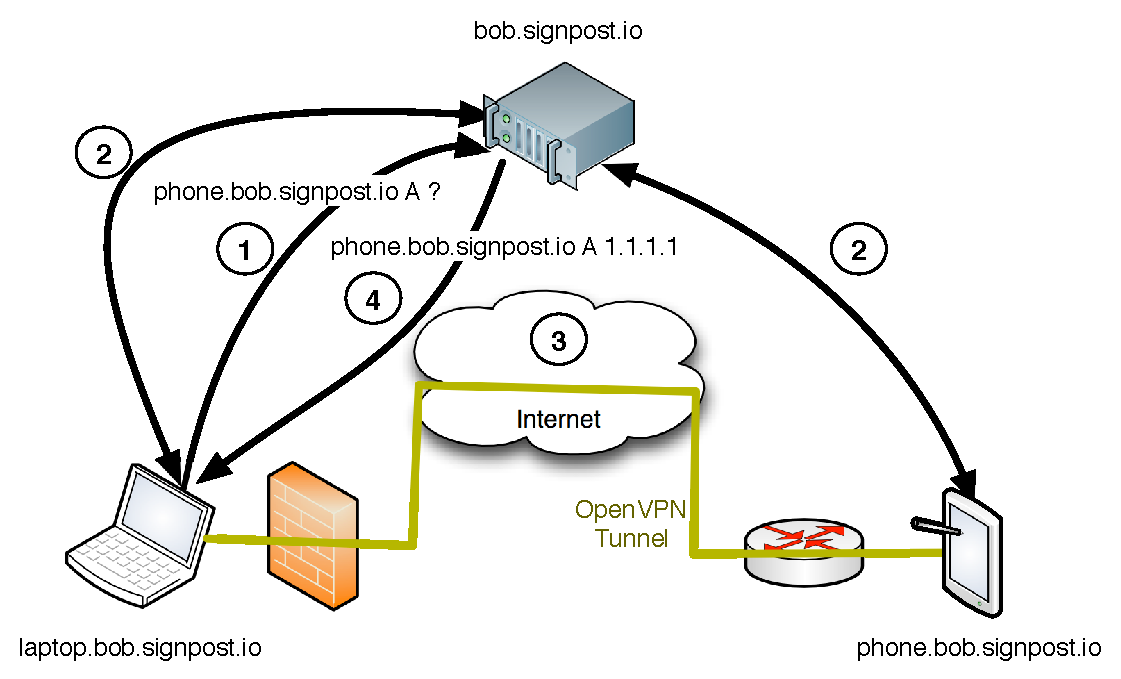
\includegraphics[width=0.6\textwidth]{Chapter3/Chapter3Figs/sp-illustration}
  \end{center}
  \caption[\signpost example use-case.]{An example use-case of the \signpost
    abstraction. Alice establishes a direct communication channel between
    her smartphone and her home PC over the Internet.}
  \label{fig:signpost-user-abstraction}
\end{figure}

In order to introduce the reader to the \signpost abstraction, 
Figure~\ref{fig:signpost-user-abstraction} depicts a simple use case example.  In this
scenario, Alice, while at work, wishes to access
files from her laptop, situated behind a home router, through her smartphone. In order to express
her interest in connecting to her laptop, Alice performs a name lookup for the domain
name \fqsn{laptop.bob} to her local \signpost resolver~(step~\ding{192}).  The
name request propagates through the public DNS infrastructure to her \signpost
cloud service, which we call the {\it \signpost controller}. A verified name
request to the \signpost controller initiates the connection establishment logic
of the system, which triggers the two devices to try multiple connection
establishment mechanisms and setup an end-to-end path~(step~\ding{193}). Once an
initial path is available~(step~\ding{194}), the controller replies to the
initial name request with a local \signpost-specific IP address. Traffic to this
address is routed by the device network stack to the established inter-device
network path~(step~\ding{195}).  In parallel, \signpost will continue to evaluate
different connection mechanisms, aiming to discover paths with higher
performance, and monitors path availability, thus recovering automatically
from disconnections. 

\section{\signpost Architecture}\label{sec:signpost-architecture}

\begin{figure}
  \begin{center}
	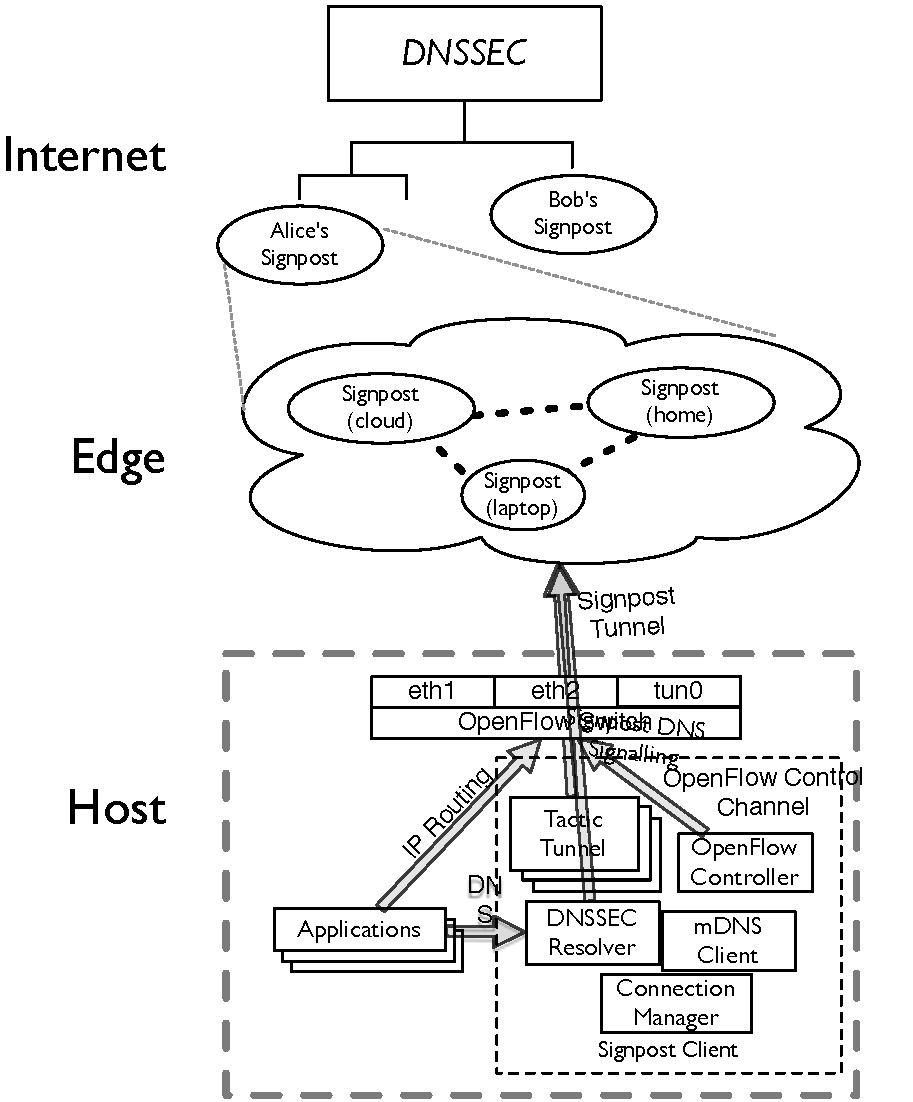
\includegraphics[width=0.9\textwidth]{Chapter3/Chapter3Figs/signpost-arch}
  \end{center}
  \caption[\signpost architecture.]{\signpost architecture presented from three different
    perspectives: The user device, the Internet, and the naming hierarchy.}
  \label{fig:signpost-arch}
\end{figure}

Figure~\ref{fig:signpost-arch} presents the architecture of \signpost from three
different viewpoints.  In the lower section of the figure, we present the design
of \signpost and its integration with existing applications.
\signpost logic is contained in a single executable, and requires the guest
OS to expose a flow control abstraction, like \of, and to redirect
DNS queries to the embedded DNS resolver.  The software consists of three
subsystems: The \textit{Connection Engine}~(Section~\ref{sec:sp-engine}),
responsible for setting up and managing \textit{Network
  Tactics}~(Section~\ref{sec:sp-tactics}) in order to establish end-to-end paths,
the local DNS resolver, and the \of-based \textit{\signpost
  router}~(Section~\ref{sec:sp-forwarding}), which enhances the normal OS routing
functionality with \signpost network control logic.
%%
The middle section of Figure~\ref{fig:signpost-arch}, presents the inter-device
connectivity architecture of \signpost. The system sets up an Internet-wide
inter-device control channel, enabling capability and parameter negotiation
between devices. The architecture  uses a special \signpost node, which we call
\emph{\signpost Controller}, to run on a well-connected host and bridge the
device control channel across the Internet, effectively orchestrating connection
negotiation and establishment.
%
The upper section of Figure~\ref{fig:signpost-arch} presents the naming
organisation of the \signpost architecture. The system reuses the naming
abstraction of the DNS service. Each device has a global domain name, while the
domain hierarchy and name aliasing expresses the control relationship between
devices and users.  We extend the normal name resolution functionality of the
DNS protocol and introduce an \textit{effectful name resolution} functionality
for \signpost-enabled domains; a name resolution expresses user interest in
connecting to another device, and triggers the test and setup of a network
path~(Section~\ref{signpost-naming}).  In the rest of this section we present in
detail the architecture of \signpost, using a bottom-up narrative.

\subsection{Network Tactic} \label{sec:sp-tactics}

\begin{table*}
\centering 
{\scriptsize 
\begin{tabular}{|l|c|c|c|c|c|c|c| }
  \hline
  Tactic name & { Purpose}  & { Protocol} & { Connectivity} & 
  { Authenticate} & { Encrypt} &{ Anonymize} & { \signpost}\\
 %% & Comment & Source \\
\hline
Avahi       & Discover       & UDP   & -       & No     & No     & No & Yes\\
 %% & Linux-based, bonjour-compatible system for local network resource discovery
 %% & \url{avahi.org/} \\
Bonjour     & Discover       & UDP   & -       & No     & No     & No & Yes\\
 %% & Used for local network resource discovery
 %% & \url{developer.apple.com/opensource/} \\
UPnP        & Discover    & UDP   & -     & No     & No     & No & No \\
dns2tcp     & Tunnel        & DNS   & TCP   & No     & No     & No & No \\
 %% & IP over DNS & \url{www.hsc.fr/ressources/outils/dns2tcp/index.html.en} \\
DNScat      & Tunnel        & DNS   & UDP      & Yes    & No     & No & No \\
 %% & VPN with PPP & \url{tadek.pietraszek.org/projects/DNScat/} \\
HTTP-Tunnel & Tunnel        & HTTP & TCP      & No     & No     & No & No \\
 %% & uses HTTP & \url{www.nocrew.org/software/httptunnel.html} \\
iodine      & Tunnel        & DNS  & IP       & Yes    & No     & No & Yes\\
 %% & IP over DNS & \url{code.kryo.se/iodine/} \\
NSTX        & Tunnel        & DNS  & IP       & Yes    & No     & No & No\\
 %% & IP over DNS. Deprecated. Recommends iodine 
 %% & \url{thomer.com/howtos/nstx.html} \\
Proxytunnel & Tunnel        & HTTP(S) & TCP      & Yes    & Yes & No & No\\
 %% & can use both HTTP and HTTPS & \url{proxytunnel.sourceforge.net/} \\
ptunnel     & Tunnel        & ICMP    & TCP      & Yes    & No  & No & No\\
tuns        & Tunnel        & DNS     & TCP      & Yes    & No  & No & No\\
 %% & IP over DNS. Doesn't split IP packets, but sets size so small that OS does
 %%   fragmentation. Neat. Only uses CNAME for maximum compatibility with
 %%   infrastructure. Poor performance :( 
 %% & \url{www.loria.fr/~lnussbau/tuns.html} \\ 
SSH         & Tunnel         & TCP     & TCP/IP      & Yes    & Yes & No & Yes\\
IPSec       & Tunnel         & IP/UDP  & IP          & Yes    & Yes & No & No\\
 %% & In layer 4 when traversing NATS (over UDP or TCP) & \\
OpenVPN     & Tunnel         & TCP/UDP & IP          & Yes    & Yes & No & Yes\\
 %% & & \url{openvpn.net/} \\
libjingle   & Nat punch      & TCP/UDP & UDP/TCP     & Yes    & Yes & No & No\\
 %% & For punching holes. Negotiation over XMPP
 %% & \url{code.google.com/apis/talk/libjingle/index.html} \\
privoxy     & Anonymize      & HTTP    & HTTP/TCP    & No     & No  & Yes & Yes\\
tor         & Anonymize      & TCP     & TCP         & No     & Yes & Yes & Yes\\
 %% & & \url{www.privoxy.org} \\
% SMTP        & Data transfer     & 7      & TCP         & Can be & Can be & No \\
stunnel     & Encrypt        & SSL     & TCP         & Yes    & Yes    & No & No\\
TCPCrypt    & Encrypt        & TCP     & TCP         & No     & Yes    & No & No\\
\hline
\end{tabular}
\caption[List of available connection-establishing
mechanisms.]{\label{tbl:signpost-tunnels}List of available
connection-establishing mechanisms. The table presents for each mechanism, its
primary functionality, the protocol used to establish connectivity and the
layer providing connectivity, and the support of the mechanism for
Authentication, Encryption, Anonymization and \signpost integration.}
}
\end{table*}

In order to provide end-to-end connectivity, \signpost uses available
functionality from the wide range of free and open source connection
establishing mechanisms. Table~\ref{tbl:signpost-tunnels}, presents a survey of
such mechanisms along with their network requirements and security properties,
highlighting the significant diversity available between mechanisms.  For example,
some mechanisms provide connectivity, bypassing strict network policies,  other
mechanisms enhance security and privacy in end-to-end Internet paths, while a
third class enables connection automation.  Furthermore, available mechanisms
vary significantly on the operating network layer and the exposed connection
abstraction. Connection mechanisms expose connectivity over a specific transport
layer port or through a network layer device.  In terms of protocols, the
majority use UDP or TCP sockets, but some mechanisms use other network
protocols, like ICMP\@.  Finally, authentication exhibits significant diversity,
spanning from user-based authentication, using either passwords or certificates,
to simple pre-shared passphrases, while some mechanisms lack support entirely. 

\begin{figure}
  \begin{center}
	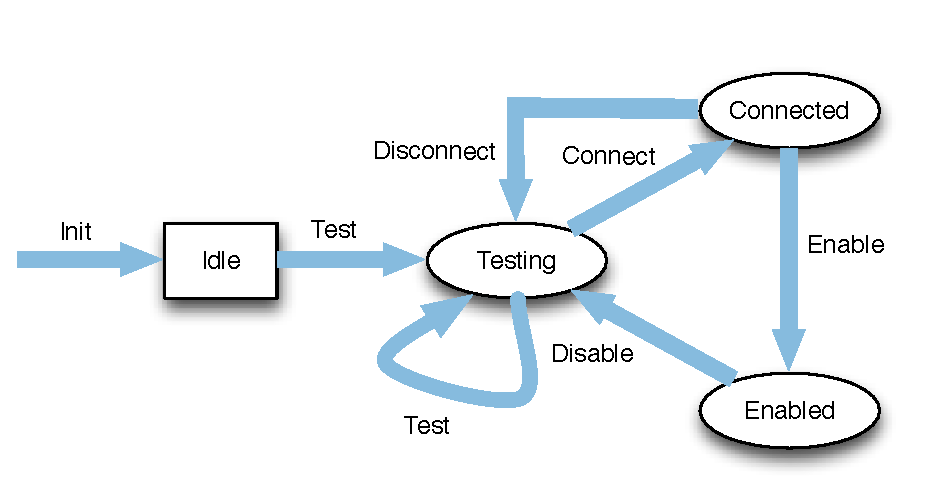
\includegraphics[width=0.8\textwidth]{Chapter3/Chapter3Figs/signpost-tactic}
  \end{center}
  \caption{\signpost Tactic lifecycle.}
  \label{fig:signpost-tactic}
\end{figure}

In order to accommodate the variances between available connection-establishing
mechanisms, \signpost defines a \textit{Network Tactic} abstraction; a generic
model encapsulating testing and control requirements and automating the
end-to-end path setup process for a connection mechanism.  A Network Tactic is
modelled as a 4 state automaton for each pair of devices, presented in
Figure~\ref{fig:signpost-tactic}.  A Tactic is initialized in the \emph{Idle}
state.  A test method invocation transfers the Tactic to the \emph{Test} state
and triggers Tactic-specific connectivity tests to discover the network policy
and configuration requirements.  If testing is successful, the Tactic can
progress to the \emph{Connected} state through an invocation of the connect
method, responsible for configuring the underlying Tactic in order to provide an end-to-end
path. Once the end-to-end path is established, the Tactic can progress to the
\emph{Enabled} state and forward traffic between the two devices over the path.
Finally, the Tactic abstraction provides methods to backtrack from each state,
tearing down any established path. 
% In order
% to avoid packet reordering, \signpost permits the parallel existence of multiple
% connected tactics for a set of devices, but a single path can be enabled at
% any point.

Furthermore, because \signpost Tactics require inter-device synchronisation and
state distribution, their functionality is distributed between the \signpost
controller and \signpost devices, and split logically into two layers: the
\emph{Southbound layer} implements low-level Tactic operations and runs on
\signpost clients; and the \emph{Northbound layer} implements the state
transitions of the Tactic automata, translating them into low-level operations,
and runs on \signpost controllers. 

The two layers of a Tactic employ the control channel between the devices and
the \signpost controller to communicate using a JSON-RPC
service~\mycite{jsonrpc}.  The control channel is exposed as a TCP service on
port 5353.  \signpost uses a control channel with high availability to
ensure Tactic parameter negotiation, even in heavily policed networks.  If
direct connectivity fails, the system uses as a fallback mechanism an
Iodine~\mycite{iodine} DNS tunnel. Iodine uses the DNS protocol to transmit
data between two hosts on UDP port 53, by encapsulating tunnel traffic in
well-formed DNS packets which can travel through recursive DNS resolvers.
Iodine can provide connectivity as long as the naming service, an important
service for Internet connectivity, is not blocked by the network. The choice of
Iodine provides sufficient capacity and latency to support the \signpost
control channel, while better integration of control messages with the DNS
packet format can improve the channel performance. 

In order to present the separation between the two layers, we present the
implementation details of the  \openvpn Tactic test method. For the specific
functionality, the Southbound layer of the Tactic provides two operations: the
\textit{init} operation, initializing an \openvpn server; and the \textit{test}
operation, testing client connectivity to an \openvpn service. The Northbound
test method uses Southbound operations to evaluate connectivity between two
devices. During connection testing between two devices, the test method will execute
in
parallel on both devices: initially, the init operation and then the test
operation towards the other device.  The first device returning a successful test
result becomes the client of the \openvpn tunnel.  If the test times-out or both
devices return a negative result,  then the controller will initialise a local
\openvpn server and execute the test operation on both devices towards the
controller.

\subsection{Forwarding} \label{sec:sp-forwarding}

\signpost exposes connectivity on the network layer of the host, thus achieving
backwards compatibility with existing decentralized applications. A \signpost
cloud is abstracted as a local subnet and each device is assigned a persistent
local IP\@. An ARP proxy, integrated with the \signpost agent,
replies with the MAC address \texttt{fe:ff:ff:ff:ff:ff}\/ to all \signpost-local
IP addresses, thus reducing broadcast traffic and focusing forwarding decisions
on the network layer.  \signpost relies on programmable network control
mechanisms, like \of, to dynamically define forwarding policy and
detect connection problems.

The majority of the \signpost control logic is defined by Network Tactics.
Non-\signpost traffic is forwarded based on the routing configuration of the
host.  For \signpost traffic, control is delegated to Tactics, which are
responsible for installing appropriate forwarding rules.  Tactics can inject
and intercept traffic and exercise control pro-actively or reactively.
Section~\ref{sec:sp-implementation} presents the  integration details between
\signpost and connection-establishing mechanisms, and elaborates on different
network control approaches.

\subsection{Connection Manager} \label{sec:sp-engine}

\signpost Tactic management is implemented by the \textit{Connection Manager}
module.  The module runs on the \signpost controller, controlling path
establishment, selecting optimal paths between device pairs and ensuring
connectivity.  Path establishment uses the Tactic abstraction to isolate
low-level connection details.  In terms of path selection, \signpost can
establish multiple end-to-end paths between two devices, but multipath
connectivity is not supported by popular transport protocols, while newer
multipath-enabled protocols, like SCTP~\mycite{RFC3286} and multipath
TCP~\mycite{RFC6824}, are not yet available in production systems.  As a result,
\signpost can use only a single end-to-end path between each pair of devices.
Path search is initiated by the connect method of the Connection Manager module,
using as parameters the device names and a list of security properties. Path
selection takes under consideration two aspects: performance and security
properties.

Path performance in \signpost reflects the resource availability in a path. The
current implementation of \signpost uses a set of simple and static heuristics
to predict path performance, based on the properties of the underlying Tactics.
More specifically, Tactics using the \signpost controller as a path relay exhibit
lower performance in comparison to direct paths, while Tactics using
connectionless protocols, like UDP, are considered more efficient than Tactics
using connection-oriented protocols, like TCP\@.  These simple rules provide an
approximation of the Tactic performance.  Path performance characterisation can
also incorporate active network measurements to improve flexibility and
estimation accuracy. 

In terms of security properties, \signpost considers three elementary
functions for each Tactic: \textit{encryption}, \textit{authentication}
and \textit{anonymity}.  An encrypted Tactic applies strong cryptography on both
directions of the path, while an authenticated Tactic uses strong authentication
during the establishment of the path.  Finally, an anonymising Tactic provides
built-in user identity obfuscation on the path.  Each Tactic provides a subset
of these functionalities, based on the capabilities of the underlying connection
mechanism (Table~\ref{tbl:signpost-tunnels}), and there is no single Tactic
that supports all security properties, and ensures connectivity under any network
environment. In order to address this limitation, \signpost defines a
\textit{Tactic synthesis} operation; a path that can be constructed by layering
multiple connectivity mechanisms and effectively create a path providing the
aggregate security properties. For example, an anonymised and authenticated path can
be established using an SSH tunnel over a TOR circuit between the two devices.
It is important to point out at this point that \signpost uses existing
frameworks to enhance security for an end-to-end path and does not develop a
security framework from scratch. The security properties of a path are a side
effect of the used Tactics.  End-users can use security properties to define
security policies towards specific devices. The policy is expressed through a
configuration file and users specify security requirements on a per domain
basis. 

Path selection is modelled as a dynamic optimization problem with security
requirements modelled as constraints and path performance modelled as the
objective function.  Path performance is represented by a positive integer
weight, with higher values reflecting lower performance of the path. The weight
of a path is equal to the sum of the individual weights of the Tactics
synthesizing the path.  Path selection uses a breadth-first search mechanism
over the complete space of all possible Tactic combinations.  During a
connection request the system spawns a thread for each Tactic, testing
end-to-end connectivity.  If the test is successful, the Tactic will try to
connect the two hosts. If the connection is also successful, and there is either
no other Tactic enabled or the enabled Tactic has a higher performance value,
then the Manager will progress the state machine of the Tactic to the
\emph{Enabled} state, and disable any existing enabled Tactics. If the Tactic
doesn't fulfil the security policy, the Manager will recursively try to layer
more Tactics over the established path and find a Tactic synthesis with
sufficient security properties. The Manager returns a successful result when the
algorithm finds a path configuration fulfilling the security policy, but the
search will continue to search for better paths.  The search will terminate when
all remaining Tactic combinations have a higher performance weight or they are
synthesized by more than three Tactics.  Effectively, the search algorithm
rapidly establishes a first path between two devices, and progressively optimizes
path performance while the devices remain interconnected. 

Finally, the connection manager  module is additionally responsible for monitoring
enabled paths and detecting disconnections. The module uses \texttt{flow\_stats}
\of messages to identify packet transmissions during a monitoring period, and
thus infer path liveness. If the path is idle during that period the
module uses a UDP heartbeat service to verify path connectivity. During a
heartbeat timeout, the connection manager tears down the path and repeats the
path search  process.  A Tactic can employ application-specific
connectivity evaluation mechanisms, e.g. \openvpn provides a keep-alive mechanism.

\subsection{Effectful Naming} \label{signpost-naming}

The majority of Internet-connected devices are essentially anonymous from a
network perspective, being assigned transient names (e.g.~via DHCP). The IPv6
protocol~\mycite{RFC1883} addresses a number of such limitations, but the protocol
deployment on the edges of the Internet has been slow and limited. A fundamental
goal for the \signpost architecture is to support stable and secure resolution
of device  names to concrete end-to-end paths.  \signpost uses the DNS
protocol~\mycite{RFC1034} to support its naming functionality for two reasons.
Firstly, DNS is an effective solution to the naming problem. It is an
Internet-wide service, supported by all network applications and never blocked
in a network. The introduction of the \dnssec protocol extensions provides
additional bi-directional authentication.  Secondly, the DNS service inherently 
supports delay-tolerant service indirection, used extensively across the
Internet.  Many services employ user-friendly domain names to represent virtual
service end-points which are refined during name resolution, directing users to
the best service mirror based on the end-host location and the service
load~\mycite{RFC3568}. Effectively, a domain name resolution represents the
interest of a user in connecting to a service, which the service provider can
direct to a concrete end-point based on the network context.  

The Internet naming service provides good scaling properties, using a
hierarchical architecture. Every domain name consists of a sequence of name
tokens organised in a hierarchical tree structure with a single root: the empty
string. Every node on the tree can be coupled with a number of DNS Resource
Records (RRs) and provides rich information on the domain name, like its network
addresses and name aliases. In order to scale the performance of the naming
service across the Internet, the design of the system allows service delegation
for a zone to other servers using the NS RR type.  In addition, the DNS
service defines a record caching mechanism, in order to improve lookup performance and
service load. 

A DNS packet (queries and responses)  contains a standard header and four
sections: the \emph{question}, containing the name being looked up; the
\emph{answer}, containing RRs answering the question; the \emph{authority},
pointing to an authoritative server for the question; and the \emph{additional}
records, containing any additional information pertaining to the question. Name
resolution then follows one of two paths. A \emph{recursive resolution} occurs
when the server does not have the answer and so it acts as a resolver itself,
pursuing the answer on behalf of the client. In contrast, an \emph{iterative
  resolution} occurs when the server does not have the answer and responds by
referring the client to a server ``closer'' to the answer.

\signpost reuses the DNS naming service abstraction and extends its
functionality, introducing the idea of \textit{effectful name resolution}.
Effectful name resolutions have as a side-effect  the creation of an end-to-end
path towards the requested destination.  Effectively, \signpost perceives name
resolutions as an intention to connect to the requested device and translate the
name resolution in an explicit connection request to the Connection Manager
module. This extension to DNS functionality is similar to the indirection
functionality of the protocol. In addition to pointing the requester to an
appropriate network address, \signpost ensures a path towards that address. 

% \begin{itemize}
% \item\emph{Ubiquity}. DNS is among the most widely deployed services on the
%      Internet. Effectively every Internet-connected client supports name
%      resolution, and has access to the DNS when connected. 
% \item\emph{Reach}. As such a critical part of the Internet's infrastructure, and
%      unlike TCP, HTTP and similar protocols, DNS tends not to be manipulated by
%      middleboxes other than modified DNS servers
%      themselves~\mycite{rfc:3234,handley-mbox}.
% \item\emph{Security}. The DNSSEC security extensions have recently been deployed
%      on the live root servers~\mycite{rfc:4033}.  DNSSEC provides origin
%      authentication and integrity protection for DNS records, and (along with
%      SSL) represents one of the two global public key infrastructures.
%    \end{itemize}

% Details of the DNS protocol can be found in RFC 1035~\mycite{RFC1035} and its
% many extensions and updates in the RFC repository. Before we discuss Signposts
% in detail, it is necessary to briefly recap key elements of DNS.

\paragraph{Secure Names For All Internet Users}

\begin{figure}
  \centering
    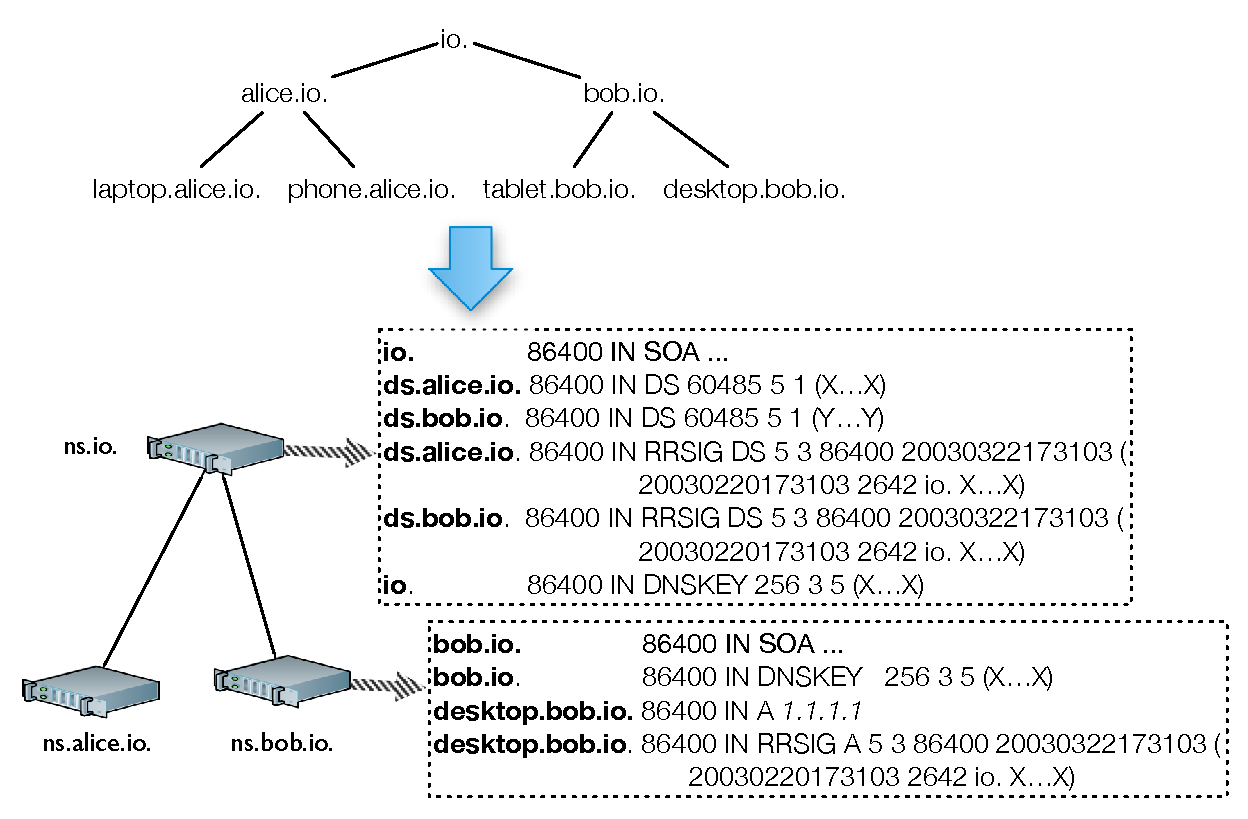
\includegraphics[width=0.9\textwidth]{Chapter3/Chapter3Figs/DNSSEC_hierarchy}
    \caption[Example \dnssec zone files.]{Example \dnssec zone files for the
        \spsn{signpost.io} and \fqsn{bob} domains. The \spsn{signpost.io} zone file
        contains a DS RR with the hash of the DNSKEY RR for \fqsn{bob}  and a
        RRSIG RR signature of the DS RR signed with the DNSKEY of the
        \spsn{signpost.io} domain. \fqsn{bob} uses its DNSKEY to sign an A RR for
        \fqsn{desktop.bob}.}
  \label{fig:dnssec_hierarchy}
\end{figure}

The initial definition of the Internet naming service provided weak security
guarantees and was vulnerable to man-in-the-middle and cache
poisoning~\mycite{DNSPoisonning} attacks.  In order to enhance the security
primitives, the IETF standardised a number of DNS protocol extensions, described
as \dnssec.  \dnssec defines four RR types~\mycite{RFC4034}, enabling response
authentication as presented in Figure~\ref{fig:dnssec_hierarchy}.  In \dnssec,
each zone owns one or more cryptographic keys to sign authoritative DNS
responses. The RRSIG RR type can carry RR signatures,
while the NSEC RR type reflects the lack of specific RRs for a domain to a
resolver.  The DNSKEY RR type disseminates public keys of a domain to resolvers,
which in turn can use them to authenticate response signatures. Finally, the DS
RR type expresses the trust of a domain to a signing key of another domain. With
respect to Figure~\ref{fig:dnssec_hierarchy}, the domain \fqsn{bob} signs an A
record for the host \fqsn{desktop.bob} through an RRSIG RR using Bob's DNSKEY\@.
Bob's key is registered with the \spsn{signpost.io} domain through a DS RR, containing the
hash of the key and signed using an \spsn{signpost.io} public key.  Effectively, the \dnssec
extensions form a chain of trust as part of the naming service and ensure
query response and key authenticity. The resolver requires, as in the X509
certificate architecture, only a list of authenticated anchors, configured
out-of-band and injected into the authentication chain.

\signpost uses the \dnssec RR types to establish an authenticated control
channel between the devices of the user. Each \signpost user must have
authoritative control of a domain zone, serviced by the \signpost controller,
and register a signing key to the \dnssec chain of trust. Each device has a
domain name under the domain  of the user. With respect to
Figure~\ref{fig:signpost-arch}, Bob is granted control of the zone \fqsn{bob}
where he registers his laptop under the domain name \fqsn{laptop.bob}. As a
result, each \signpost user has a globally accessible authenticated public
identity for each device via a public-private key-pair. Using this key-pair, a
user can sign and authenticate messages, bootstrap public key cryptography
mechanisms and run key-exchange mechanisms, such as
Diffie-Hellman-Merkle~\mycitet{RFC2631}, and derive new shared private keys
between any two devices over unsecure channels.

The base \dnssec RR types  provide a mechanism for authenticating responses from a
nameserver to a DNS resolver. In terms of the \signpost architecture, we are
additionally interested in authenticating DNS requests. Authenticated requests
enable the server to present a different view over the resource mappings,
depending on the querying entity\footnote{{\em ``DNS servers can play games.  As
    long as they appear to deliver a syntactically correct response to every
    query, they can fiddle the semantics.''---\,RFC3234~\mycite{RFC3234}}}.
\signpost uses the SIG(0) RR type, defined in~\mycite{RFC2931}, to sign DNS
requests using the key of the device.  
% The record was introduced in order to allow authorized
% clients to update RR records on an authoritative server, while it permits a
% client also to point to the signing entity, in order to fit the authentication
% within the \dnssec key structure. 

% Using DNSSEC here instead of SSL has several important advantages. Firstly,
% DNSSEC has maintained the integrity of its trust chain better than SSL (which
% has a large set of root certificate providers), and has explicit support for
% incomplete trust chains via look aside validation~\mycite{RFC5074}.  Secondly,
% DNSSEC has few network dependencies and exploits all of the distributed benefits
% of DNS, such as caching, proxy lookups, and a low-latency protocol.  Lastly, a
% domain also has a single, well-defined owner if registered under a top-level
% domain, whereas URL-based identity schemes such as
% OpenID~\mycite{Recordon:2006:OPU:1179529.1179532} depend on trusting the
% underlying owner of the domain for that URL.\todo{will we discuss icann
%   implications of so many new internet names later on?}

%% \subsection{Centralised Named Routing}
%% \label{s:topo1}

\paragraph{\signpost Integration With \dnssec} 

\signpost evolves the \signpost client and controller DNS functionality.
Specifically, the controller runs a programmable DNS service, which is
authoritative for the user domain. The server is authoritative for the
user domain zone,  signs responses on-the-fly, verifies SIG(0) signed queries, and
translates them into Connection Manager requests. A request for an A RR for
domain name \fqsn{laptop.alice}, signed with a SIG(0) record with a key from
host \fqsn{desktop.alice}, will be translated into a connection request between
Alice's laptop and desktop devices.  
% In order to enforce liveness of \signpost
% RR records in the Internet, we set a zero TTL value on all RR records, thus
% disabling any DNS caching.
In the client side of the \signpost architecture, we use a local \signpost-aware
DNS resolver. DNS queries for non-\signpost hosts trigger a recursive search of
the DNS name tree, in order to retrieve the requested RRs.  For \signpost 
requests, the resolver signs the query with a SIG(0) record using the private
key of the device. 

DNS provides additionally offline functionality in a local network.
Specifically we use DNS-based service discovery~(DNS-SD)~\mycite{RFC6763}, an
RR organisation specification which enables service advertisement and browsing
in a local network. DNS-SD uses the Multicast-DNS~\mycite{RFC6762} service and
provides an efficient local service discovery mechanism. The combination of
DNS-SD and multicast-DNS is currently a popular service discovery mechanism in
local networks, supported by most operating systems.  \signpost
advertises, using the DNS-SD mechanism, a \signpost service record with name
\spsn{\_sp.\_tcp.local} along with an RRSIG RR and the DNSKEY RR of the device,
signed with the private key of the user domain. Another \signpost client can
verify a \signpost service, using a locally cached copy of the
\signpost controller public key, and establish a control channel.  In offline
mode, a query receiver functions as a \signpost controller, responsible for the
server RR request for its domain name only.

\subsection{Security and Key Management} \label{signpost-security}

\signpost extends the \dnssec architecture to develop a public key
distribution mechanism.  Firstly, \dnssec exhibits better trust chain integrity
in comparison to SSL, which has a large set of root certificate providers, and
supports incomplete trust chains via look aside validation~\mycite{RFC5074}.
Secondly, a domain in \dnssec has a single, well-defined owner, registered under
a top-level domain, whereas URL-based identity schemes, like
OpenID~\mycite{Recordon06}, are subject to the trust to the domain owner.

\signpost key hierarchy extends the \dnssec key hierarchy and introduces an
additional layer of device keys in each user domain. \dnssec deployment
specifications dictate the use of at least two RR signing
keys~\mycite{RFC4641}: A \textit{Zone Signing Key (ZSK)} and a \textit{Key
Signing Key (KSK)}.  ZSK signs the KSK, and its hash is stored as a DS RR in
the top-level zone. KSK is used by the controller to sign authoritative RRs\@.
The use of two keys by the authentication mechanism provides a persistent
anchor in the \dnssec key hierarchy for each domain and enhances flexibility in
key revocation; KSK rollover requires only a few record modification in the
zone file.  \signpost introduces an additional layer of \textit{Device Signing
Keys (DSK)}, which are signed using the KSK and used by the devices to
bootstrap authentication.  In order to join a Personal Cloud, a device must
generate a DSK and add it in the zone file of the \signpost controller using a
DNSKEY RR and a signed RRSIG RR\@. Any device with an anchor in the global
\dnssec key infrastructure can verify any \signpost signed request, by
following the key chain in the \dnssec tree.

\section{Evaluation}\label{sec:signpost-evaluation}

In this section we evaluate a strawman implementation of \signpost and its
compatibility with distributed Personal Cloud applications.  Specifically: we
present a strawman \signpost implementation and its integration with a set of
Tactics (Section~\ref{sec:sp-implementation}); we measure the performance of
the available \signpost Tactics in a representative testbed
(Section~\ref{sec:sp-tactic-eval}); and we discuss the experience in the
integration of \signpost with a set of popular applications
(Section~\ref{sec:sp-compatibility}). 

\subsection{\signpost Implementation} \label{sec:sp-implementation}

\signpost is implemented predominantly in OCaml, a type-safe functional
language providing enhanced security and fast prototyping.  The implementation
uses existing protocol libraries to integrate programmable protocol support for
\dnssec and \of. Our strawman implementation is fully functional under Linux
and Android, using the \ovs switch implementation, and MacOSX, using the
ocaml-openflow library userspace switch implementation. The \signpost
implementation supports  the following connection-establishing mechanisms: 

\begin{itemize}

    \item \emph{Direct}: The Direct Tactic evaluates the ability of  two devices
        to connect directly without any tunnelling mechanism. The Tactic test method
        evaluates if direct bi-directional connectivity is possible between the two
        devices on a set of well-known service ports (e.g. TCP and UDP connectivity
        on ports 53, 80, 443 and 8080). If the tests are successful, the Tactic
        inserts \of rules on both devices to translate \signpost addresses into
        network addresses. 

    \item \emph{\openvpn}: The \openvpn Tactic integrates the respective
        tunnelling mechanism with \signpost. The Tactic test method evaluates
        inter-device and device-\signpost controller connectivity on UDP port 1194.
        The Tactic connect method uses the \signpost keys to bootstrap the \openvpn
        authentication mechanism.  Because of some limitations in OpenSSL certificate
        chain evaluation, for each path the Tactic generates transient private keys,
        signed by the user private key, and injects in the trusted certificate
        configuration of the \openvpn software a certificate for the destination
        device key signed by its private key.  The Tactic configures the \openvpn
        software to expose connectivity through an Ethernet TAP
        interface~\mycite{tuntap}, which is added to the local switch datapath. Each
        TAP device is assigned an IP in the 10.0.0.0/16 subnet and appropriate ARP
        announcement packets are broadcast, to bootstrap state in the internal
        \openvpn ARP cache. Finally, The Tactic enable method inserts \of rules to
        forward packets over the \openvpn tunnel and translate source and destination
        addresses, similarly to the direct Tactic.

  \item \emph{SSH}:  The SSH Tactic provides inter-device connectivity using the SSH
    protocol. The Tactic configures and runs an SSH server on every \signpost
    device on port 10000, configured exclusively to provide tunnelling
    functionality using key-based authentication. The Tactic spawns a separate SSH
    daemon on each device, to enable tighter service configuration.  Tactic
    testing evaluates direct TCP connectivity between the devices or through the
    \signpost Controller.  The connect method of the SSH Tactic appends the
    public key of the destination device in the \texttt{authorized\_key} and the
    \texttt{known\_host} SSH configuration files and uses the device private key to
    authenticate the client and server during connection.  The SSH Tactic
    associates the SSH tunnel with a local TAP Ethernet interface on each device
    and the Tactic inserts appropriate \of rules to forward traffic to the TAP
    interface.

\item \emph{Privoxy}: The Privoxy Tactic enables HTTP request anonymisation
    using the~\mycitet{privoxy} HTTP proxy. The Tactic provides a mechanism
    for purging HTTP requests and responses from user identification elements, but
    does not ensures connectivity. The Tactic test method configures a
    Privoxy HTTP proxy server on each device, configured with a strict
    anonymisation policy, and succeeds only when the Tactic is used in a synthesised
    path and the Tactic is tested over an existing connection-establishing Tactic
    (e.g.~direct, \openvpn,~etc.). The Privoxy connect method handles TCP flows in a
    proactive manner.  For each SYN packet, the Tactic installs bi-directional
    flows, forwarding data from the application to the local listening port of the
    Privoxy daemon.

\begin{figure}
  \begin{center}
	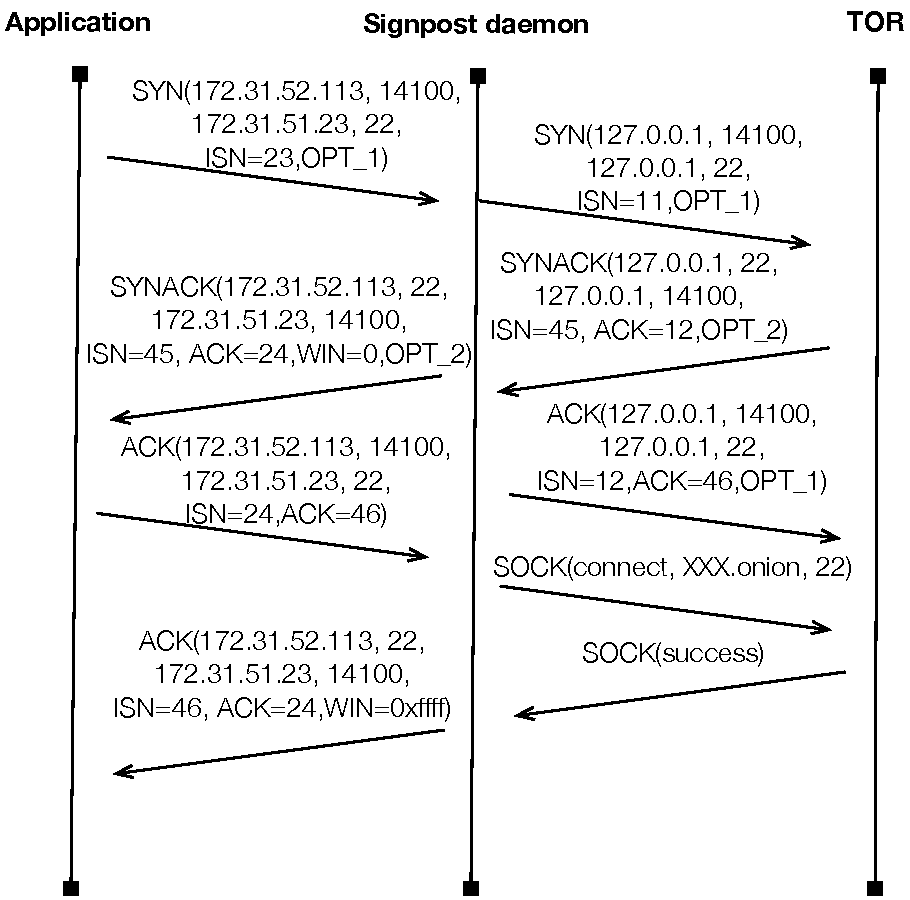
\includegraphics[width=0.7\textwidth]{Chapter3/Chapter3Figs/tor-example}
  \end{center}
  \caption[TOR Tactic connection establishment sequence diagram.]{TOR Tactic
    connection establishment sequence diagram. The Tactic translates each
    TCP connection request to a \signpost device into a SOCKS
    request to the TOR proxy.}\label{fig:signpost:tor-example}
\end{figure}
  
  \item \emph{TOR}: The TOR Tactic enables connectivity between devices over the
    TOR anonymised network~\mycite{dingledine2006}. The Tactic configures a TOR
    client on each device, exposing a SOCKS proxy and uses the TOR hidden
    service functionality to support inter-device connectivity. The Tactic
    generates for each host an anonymised domain name under the \spsn{.onion}
    domain and employs the embedded name lookup capability of the SOCKS protocol
    to provide host discoverability over end-to-end TOR circuits. The TOR test
    method initializes the TOR client, propagates the domain name of the device
    to the \signpost controller and tests the effectiveness of the Tactic in the network
    environment.  
    
    The TOR Tactic uses a reactive control scheme. For each SYN packet to a
    \signpost host, the Tactic injects packets to initiate a TCP connection
    with the local SOCKS proxy and sends a SOCKS request to establish a TOR
    circuit to the destination device.  On TCP connection establishment with
    the local SOCKS proxy, the Tactic responds to the initial SYN request with
    a SYNACK packet with sequence and ACK numbers which accommodate the
    additional bytes of the SOCKS request, and a zero receive window, to
    suppress any further data transmissions from the application.  Once a
    positive SOCKS response is received, the Tactic sends to the initiating TCP
    flow an ACK packet with a non-zero window and insert appropriate \of rules
    for in-kernel IP addresses and port numbers translation. On negative SOCKS
    response, the Tactic injects TCP RST packets in order to tear-down all
    flows. Figure~\ref{fig:signpost:tor-example} presents a sequence diagram of
    the Tactic interactions.  In order to replicate a similar abstraction for
    UDP and ICMP traffic, we setup a~\mycitet{vtun} tunnel over TOR, thus
    enabling IP-level connectivity.  We avoided using the tunnel for TCP
    connections in order to reduce header capacity losses of the tunnelling
    mechanism.

  \item \emph{DNS-SD}: The DNS-SD Tactic enables service advertisement between
    \signpost devices. DNS-SD~\mycite{RFC6763} is a common OS service enabling
    hosts to advertise services in the local network.  The Tactic aids existing
    decentralised Personal Cloud applications to discover available services
    running on other \signpost devices. Similarly to Privoxy, the Tactic does
    not provide connectivity and thus can only be used in synthesized paths.
    The Tactic connect method intercepts DNS-SD packets from the network stack
    of the device and propagates them over the control channel to the other
    devices of the user.  \signpost daemons inject equivalent DNS-SD multicast
    packets through the \of protocol to the network loopback device and thus
    provide service discovery.

\begin{figure}
  \begin{center}
	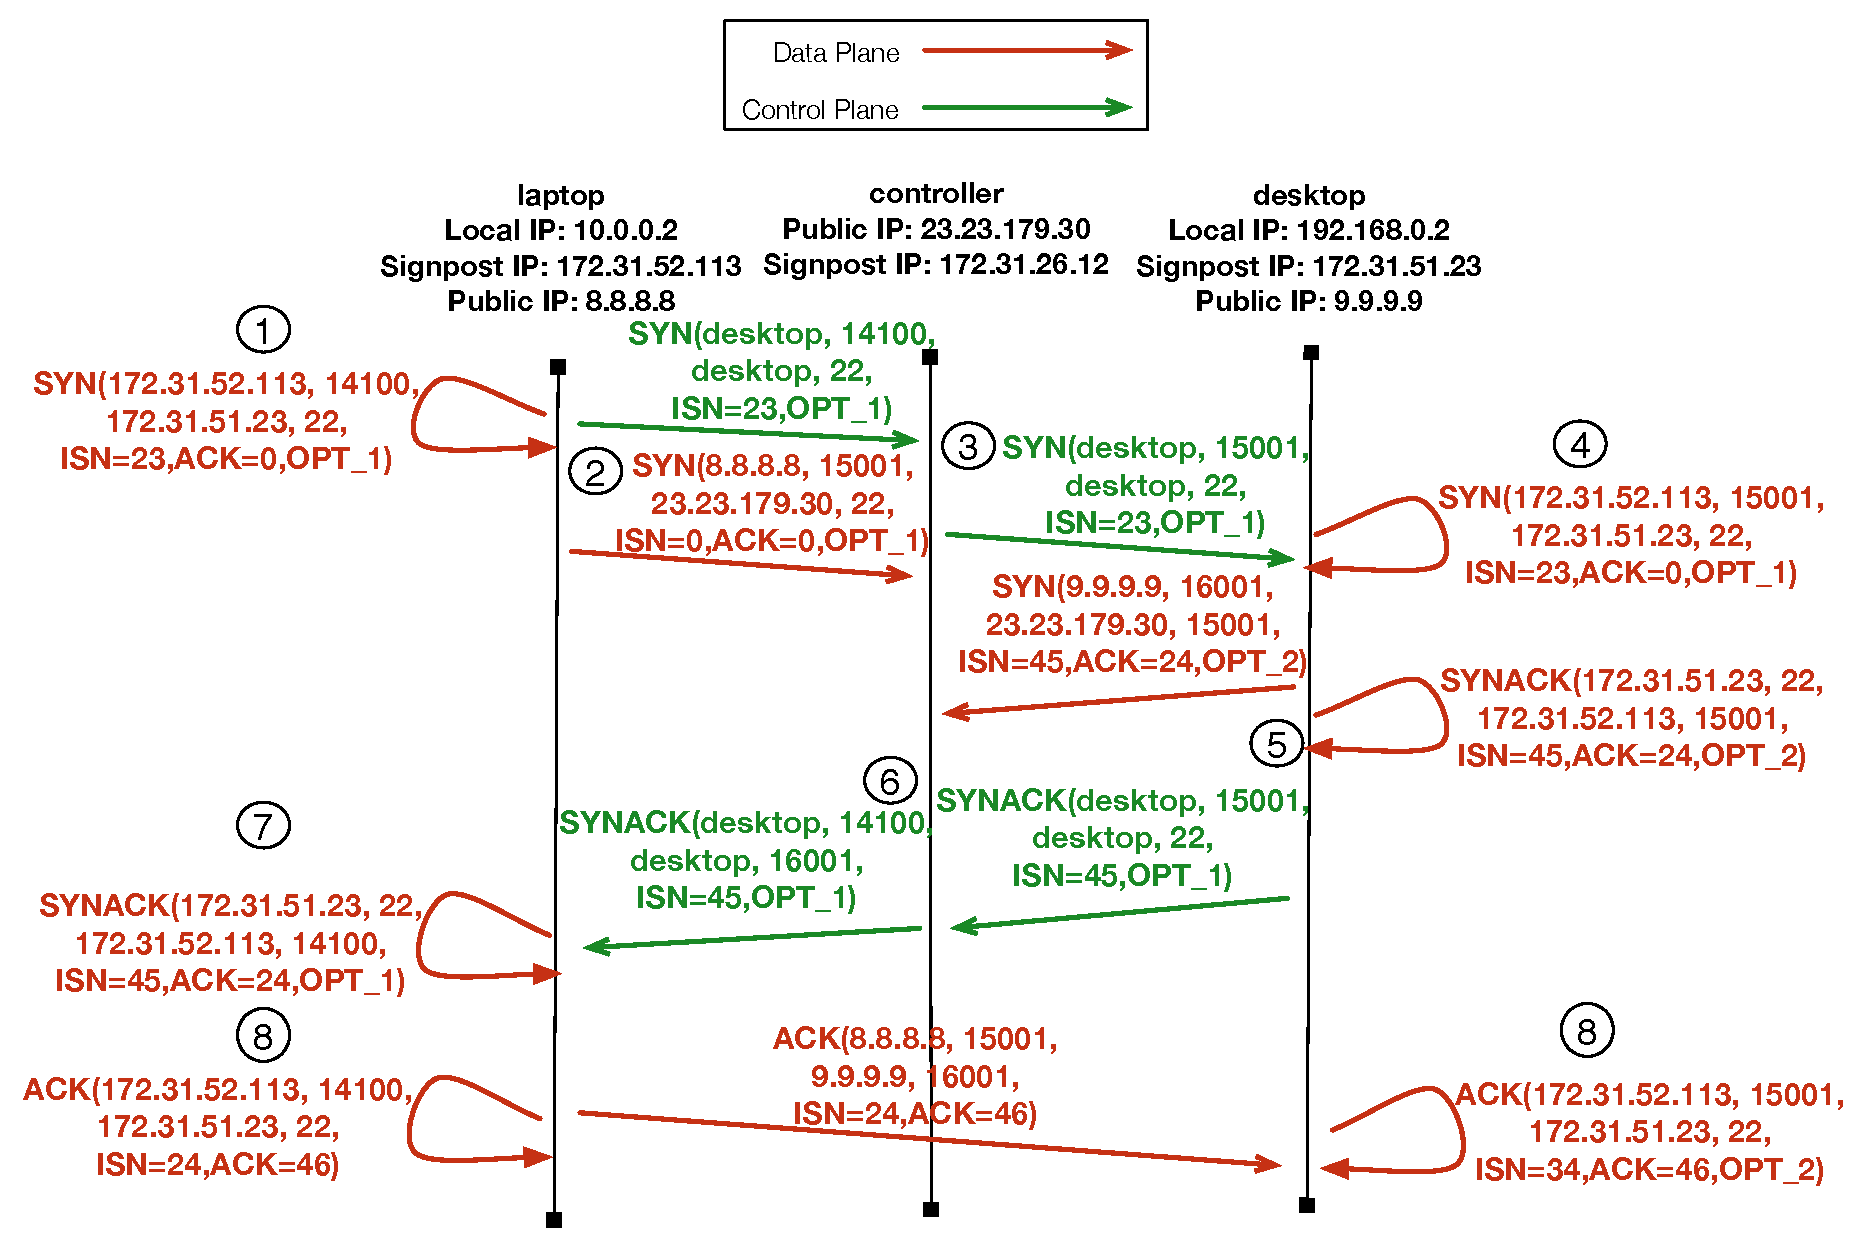
\includegraphics[width=0.99\textwidth]{Chapter3/Chapter3Figs/nat-punch-example}
  \end{center}
  \caption[NAT-punch Tactic connection establishment sequence
  diagram.]{NAT-punch Tactic connection establishment sequence diagram. The
  Tactic injects crafted packets to create appropriate state in the local NAT,
  while the controller detects the applied port mapping for both hosts of the
  \signpost path.}
  \label{fig:signpost:nat-panch-example}
\end{figure}
  
  \item \emph{NAT-punch}: The Tactic implements a packet injection technique which
    allows TCP and UDP flows to bypass NAT boxes. The Tactic supports only
    Full-cone NAT, Address-restricted NAT and Port-restricted
    NAT~\cite{RFC3489}.  The NAT-punching Tactic uses the \signpost controller to infer
    the port mappings configuration of the local NAT\@. We present a sequence
    diagram between two devices and the \signpost controller in order to establish a TCP
    connection using the NAT-punch Tactic~\ref{fig:signpost:nat-panch-example}.
    Specifically, for a new TCP connection, the daemon intercepts the SYN packet
    (Step~\ding{192}), propagates important header fields~(Port number, initial
    sequence number and TCP options) over the control channel to the remote
    device and sends a SYN packet from the device to the \signpost controller, in
    order to infer the port mapping policy and create the appropriate state in the
    NAT (Step~\ding{193}). When the \signpost controller receives the SYN, it
    extracts the source port mapping applied by the NAT and forwards it, along
    with the TCP initial sequence number, to the destination device
    (Step~\ding{194}).  Once the destination device receives the control message
    from the \signpost controller, it will generate a SYN packet, using the header fields
    of the initial SYN packet, and send both to the listening service and the
    \signpost Controller~(Step~\ding{195}). In the destination device, the
    \signpost daemon intercepts the SYNACK response of the listening service and
    propagates the TCP header fields over the control channel to the connection
    initiating device~(Step~\ding{196}).  Once the exact port-mapping is
    inferred by the Controller, the information is propagated to the initiating
    device~(Step~\ding{197}), which will inject a SYNACK packet to the local
    stack to progress the TCP-handshake~(Step~\ding{198}). Finally, once the two
    devices know the NAT port-mapping and have created the appropriate state in the
    NAT flow table, the Tactic inserts \of rules to translate appropriately
    incoming and outgoing traffic of the flow~(Step~\ding{199}).

    For UDP traffic, the Tactic controller will intercept the initial UDP packet
    of the flow and propagate it over the control channel to the remote device,
    as well as transmit a similar packet to the \signpost controller in order
    to generate the appropriate state in the intermediate NAT services. The remote
    device sends a similar UDP packet to the \signpost controller. Once the
    controller has received both UDP packets, it will notify both devices to
    appropriately transform flow IP address and port numbers, using \of flows. 
\end{itemize}

\subsection{Tunnel Evaluation} \label{sec:sp-tactic-eval}
\begin{figure}
  \begin{center}
	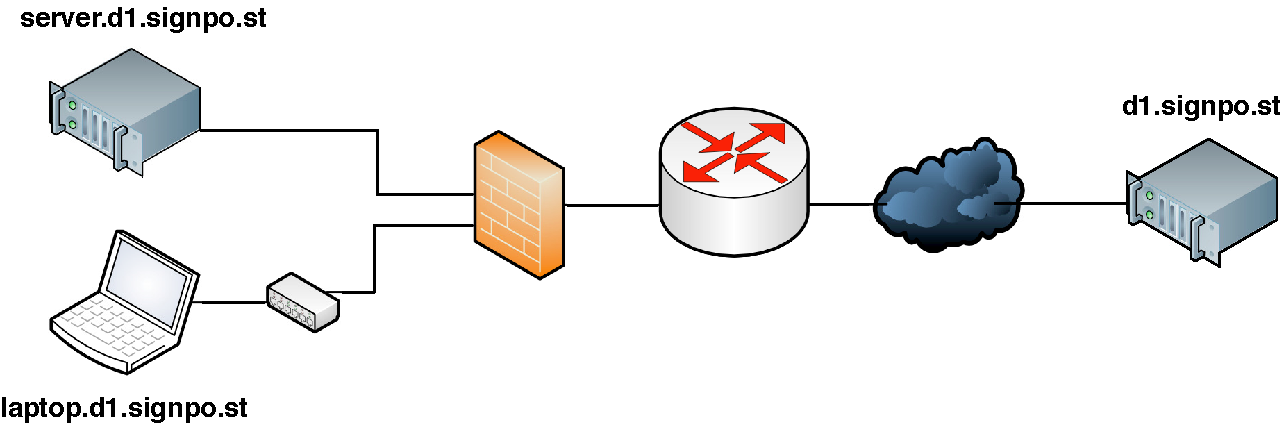
\includegraphics[width=0.9\textwidth]{Chapter3/Chapter3Figs/measurement_topology}
  \end{center}
  \caption[\signpost Tactic evaluation topology.]{\signpost Tactic evaluation
    topology. \textit{server} and \textit{laptop} hosts are connected on
    different subnets of the CL network. The laptop is connected to the network
    through a NATed home router and a stateful firewall enforces network policy
    between the two subnets.  The \signpost \textit{controller} is hosted on an
    Amazon EC2 micro instance~\mycite{ec2instances}.}
  \label{fig:signpost:measurement_topology}
\end{figure}
 
\begin{table}
\centering
\begin{tabular}{|l|>{\centering\arraybackslash}m{1.2cm}|>{\centering\arraybackslash}m{1.7cm}|>{\centering\arraybackslash}m{1.5cm}|>{\centering\arraybackslash}m{1.2cm}|>{\centering\arraybackslash}m{1.7cm}|>{\centering\arraybackslash}m{1.5cm}| }
  \hline
  \multirow{2}{*}{Tactic name} & \multicolumn{3}{|c|}{Direct Connectivity} &
  \multicolumn{3}{|c|}{Cloud-assisted Connectivity} \\
\cline{2-7}
& setup (sec) & throughput (Mbps) & RTT (msec) & setup (sec) &
throughput (Mbps) & RTT (msec) \\
\hline
Direct       & 1.0  & 94.1 & 1.5   & -    & -     & -     \\
\openvpn     & 13.3 & 66.0 & 1.23  & 20.0 & 1.9   & 172.0 \\
SSH          & 6.8  & 86.5 & 2.73  & 8.8  & 1.7   & 829.0 \\
TOR          & 60.2 &  2.4 & 912.0 & -    & -     & -     \\
NAT-punch    & 1.2  & 94.1 & 1.5   & -    & -     & -     \\

% iperf -c quorum101.cl.cam.ac.uk  -i 1 -F /dev/urandom -t 60
% fping 172.31.28.49 -e -b 1400 -c 6000 -p 1 -D -s -e -q
\hline
\end{tabular}
\caption[\signpost Tactic performance.]{\signpost Tactic performance evaluation
  results in terms of latency to setup a path, throughput and RTT delay. Direct
  cloud-assisted paths exhibit two orders of magnitude higher performance and
  lower throughput.
\label{tbl:signpost:tactic_perf}}
\end{table}

In order to evaluate the performance of our strawman implementation, we conducted
a series of measurements for each Tactic.  Our testbed consists of three hosts,
two \signpost devices and a \signpost controller, presented in
Figure~\ref{fig:signpost:measurement_topology}. The \signpost
clients~(\fqsn{laptop.d1}, \fqsn{server.d1}) are connected to the production
network of the Computer Laboratory on different subnets through 100 MbE links.
The network enforces a security policy between both devices and towards the
Internet using a stateful firewall.  Additionally, the host laptop is connected
to the network through a home router with NAT functionality. The \signpost
controller of our experiment runs on an Amazon EC2 micro
instance~\mycite{ec2instances}. Using \signpost, we establish all possible
end-to-end Tactics\footnote{We exclude the privoxy and DNS-SD Tactics because
they improve functionality on established paths only.} and measure the path
setup delay, the achievable throughput, and the round trip delay for each
Tactic. More specifically, in each experiment we initialize the \signpost
daemon on each device, and establish connectivity using a specific Tactic. For
each established path we measure the delay in completing a \signpost name
resolution and initialize a \signpost path, the path throughput, using a
steady-state TCP measurement probe, and the average path RTT, using a 1 Mbps
UDP measure probe. We conducted our measurements ten times for each possible
configuration and present the median values in
Table~\ref{tbl:signpost:tactic_perf}. 

From the results of our experiment, we note the difference in capacity and latency
when a path uses the \signpost controller. Edge network connectivity provides
two to three orders of magnitude higher performance in comparison to
cloud-assisted paths.  In addition, we highlight the trade-off between security
and performance between Tactics. For example, the TOR anonymisation
functionality significantly degrades performance and latency, deeming it
inadequate for responsive applications. The performance degradation is primarily
due to the onion routing scheme used to obfuscate the source and destination
addresses of the flow, and the sharing nature of the system.  \signpost exposes a
clear control abstraction of the trade-off between performance and security. 

An important aspect of Tactic performance is the path setup latency. This delay
is important because the DNS protocol employs time-outs in name resolutions to
detect unresolvable domain names. Linux and OSX have a maximum delay of 15
seconds\footnote{\url{http://linux.die.net/include/resolv.h}} (3 retries with 5
seconds time-out per request), while for Windows the delay varies between 12 to
15 seconds depending on the OS
version\footnote{\url{http://blogs.technet.com/b/stdqry/archive/2011/12/15/dns-clients-and-timeouts-part-2.aspx}}.
Bootstrapping a \signpost path incurs noteworthy setup latencies, but the DNS
naming service is designed to handle such latencies.  Based on
Table~\ref{tbl:signpost:tactic_perf} results, the majority of the Tactics
exhibits setup latencies within the resolver time-out limit, except the TOR
Tactic. TOR setup latency is dominated by the circuit establishment latency of
the onion overlay.  The current implementation exposes the setup latency to
applications and thus may experience DNS name lookup time-outs for the first flow
of a path. An optimistic approach can mitigate potential resolver time-outs
(e.g.~use of DNS aliases to delay the response). It is important at this point
to clarify that the measured setup latencies occur only for the first flow
of a path, and subsequent flows will experience name resolution delays
equal to the round-trip time to the \signpost controller. 

Finally, using the aforementioned topology we also measured the performance of
Tactics synthesis. The results of the experiments report that the throughput and
RTT of such paths is equal to the minimum value between the Tactics forming the
network path, while the setup latency is equal to the sum of the individual
Tactics. 

\subsection{Application Compatibility} \label{sec:sp-compatibility}

In this section we evaluate the compatibility of \signpost with applications
providing resource and information sharing. Our evaluation focuses on the
effectiveness of \signpost integration with such applications.  We used the
topology in Figure~\ref{fig:signpost:measurement_topology} and considered two
primary classes of applications: \emph{File Sharing} and \emph{Resource
  sharing}.  In terms of file sharing, we tested three popular applications, namely
the Linux NFS implementation~\mycite{RFC5661}, git-annex~\mycite{git-annex} over
rsync and SSH Secure Copy.  In terms of resource sharing we tested the
functionality of CUPS remote printing, DAAP media sharing, VNC remote desktop
and SSH remote access. 

We report that all applications functioned correctly from a network perspective
over all Tactic configurations. Nonetheless, user-perceived performance is
proportional to the underlying Tactic performance
(Table~\ref{tbl:signpost:tactic_perf}).  Some Tactics incur significant RTT
delays and impact the user-experience in reactive applications. For example,
the SSH software exhibited significant responsiveness problem when routed over
TOR\@. In addition, through the integration testing we identified limitations
in the openness of our architecture and modified accordingly our
implementation. For example, we observed that the Linux SSH client and server
use different values for the ToS bits, depending on the payload of the packet,
and require the respective \of rule to wildcard the ToS field value in the
NAT-punch and TOR Tactics. Our design choice to integrate \signpost with
existing network applications in the network layer of the OS is effective and
enables seamless integration with existing network applications.

\section{Summary} \label{sec:signpost-conclusion}

This chapter focused on the problem of Internet-scale inter-device connectivity.
Our work is motivated by the end-user requirement for resource and information
sharing services using network device federation between its personal devices; a
generic abstraction which we termed Personal Cloud. We elaborated on the available
mechanisms and highlighted trade-offs between available solutions. We identified
a significant connectivity and naming problem in the current Internet
architecture.  We argued that the abundance of connection-establishing mechanisms
provides a sufficient toolset to connect devices across the Internet, but
requires a distributed control framework to orchestrate the automatic
establishment of end-to-end paths using these mechanisms. We presented \signpost,
a distributed naming and connectivity framework which enables global device
naming,  automates the testing and  configuration of end-to-end paths and
provides secure and backwards-compatible connectivity to existing network
applications. 

\signpost evolves two aspects of user device control plane. Firstly, the control
plane is extended to accommodate \textit{Network Tactic} functionality;
mechanisms enabling ad-hoc end-to-end connectivity, like tunnelling software and
NAT punching techniques. The architecture develops a generic model coupled with
a secure and high-availability Internet-wide control channel, enabling
inter-device Tactic testing and configuration orchestration.  In addition, the
rich security properties provided by existing network Tactics, allow the system
to expose a security control abstraction, providing trade-off control between
performance and security.  Secondly, the architecture integrates the control
plane logic with the naming service. \signpost provides Internet-wide
persistent device names and a global and secure key distribution mechanism,
building on top of the \dnssec extensions.

We presented our strawman \signpost implementation and its  integration with
network connectivity applications, and evaluated the performance of \signpost
paths and its compatibility with existing network applications. We elaborated on
the integration details of \signpost  with direct, \openvpn, TOR, SSH, Privoxy,
DNS-SD and NAT-punch software and connection techniques, supporting  the
generality of the \signpost Tactic model. Additionally, we measured the
performance of integrated Tactics in a typical deployment scenario and verified
the backwards-compatibility of the system with a number of popular decentralised
network applications. In the next chapter, we conclude the results of our research and
discuss future work directions.
